\chapter{CMS Detector}

The CMS is one of the four experiments at the Large Hadron Collider (LHC), which is the largest and most powerfull particle accelerator in the world. This accelerator collitionates protons at very high energies of the order of 13 TeV, with the objetive of studying the elemental particles of the universe. 

The LHC is conform by a ring of almost 27 km and by 4 detectors located at the different collition points of the ring. 2 of these detector are general-purpose detectors, they belong to the experiments CMS (Compact Muon Solenoid) and ATLAS (A Toroidal LHC ApparatuS). Both experiments share the same goals of searching physics beyond the SM as: search and measurement of the Higgs boson, Supersymmetry searches, DM, detection of extra dimensions, among others. The difference between both experiments is that they use different technical solutions and the magnetic field is produced by a different system design. In the ATLAS detector the magnetic field is produced by a central toroid, two end toroids and a central solenoid, while the CMS detector is built around a solenoid magnet.  

The CMS and ATLAS dectectors have a cylindrical form in order to have the most uniform magnetic field posible, they are centered in the direction of the interacting beams and the collition point and have two ``end-caps'' to cover the forward regions. These detectors are conformed by the same general components, from the inner part of the detector to the outer part, these are: a tracking system, an electromagnetic and a hadronic calorimeter and muon detectors. They also have magnets to curve the path of the electric charged particles, so it can be determined whether a particle has a positive or negative charge. Aditionally, the measurement of the curve can be used to calculate the momentum of the charged particle. In the figure \ref{CMS_detector}, there is a scheme showing the structure of the CMS detector. This image also shows the interaction of different particles with the parts of the detector.

%\section{Accelarator and Storage Ring}

 \begin{figure}[h] \label{CMS_detector}
 \centering
 \caption{CMS detector.}
 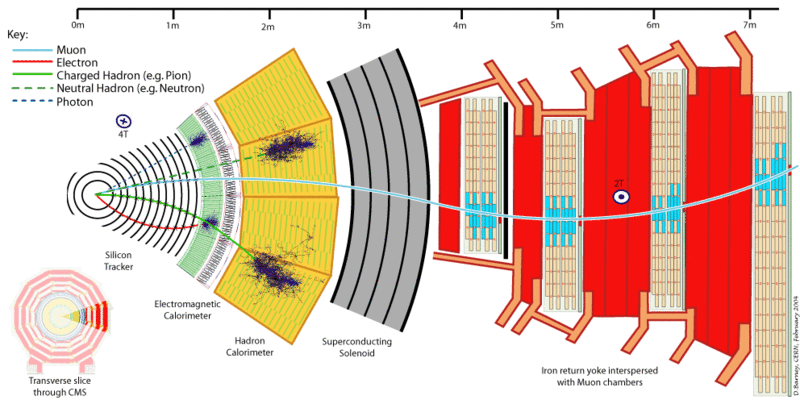
\includegraphics[width=0.9\textwidth]{./Capitulos/CMS/CMS}  
 \end{figure}

\section{Tracks Detector}

Since every 25 ns there is a collition at the center of the CMS detector, almost 1000 particles are going to be produced, so it is necessary to have a tracking system able to record measurements the nearest possible to this region. This tracking system must measure the momentum and vertices of the particles with a high precision. The inner detectors are construct with silicon detectors, with high granularity pixel systems at the smallest radii, and silicon-strip detectors at larger ones. 
%Citar libro:perspectives on LHC Physics

The properties of the tracking system are: fast taken of measurements, toleration to high radiation doses, ensembled with light material and toleration of the severe conditions imposed by the low temperature at LCH (of almost 2 K). One of the major challenges for the inner dectector parts is the control of aging effects because the damage produced by irradiation is severe. The silicon detectors are p-n junction diodes, so when a particle crosses the detector, it causes the liberation of electron-hole pairs, which move to the electrodes of the system. The tracking system in the CMS detector covers the range within $|\eta|<2.5$, the region where most of the particles arrive. 

The flux of particles arriving to a point in the detector depends of the distance from the center of collition to where the detector is located: as the flux crosses the detector material the quantity of particles decrease. Thus, the resolution of the tracking system does not need to be so high in the intermediate and end caps of if. For this reason, in the first region of the tracking system (the closest to the interaction point), there are silicon pixel detectors with cell size of $100 \times 150 \mu m^2$. THe innermost layer of pixels is located as near to the beam as it is practical, this is at a radius around 4.5 cm.
 
The silicon pixels are expensive and have high power density. Aditionally, the flux of particles at an intermediate region of the inner detectors the flux of particles is low enough to use silicon microstrip. Thus, in the region of radius greater that 20-55 cm the silicon pixels are replaced by silicon microstrip. These silicon microstrip are arranged in a special way to improve the resolution in the z axis. These barrel cylinders and end-caps dics, as the silicon pixels ,cover the region of $|\eta| < 2.5$ . The strip dimensions are or around $11 cm \times 100 \mu m$.

In the outermost region of the tracking system (at a radius greater that 55 cm) the particle flux is low enough to use a larger-pitch silicon microstrips. The maximum size of these cells is $25cm \times 80 \mu m$. There are 6 layers of these silicon microstrips moduls in the barrel and 9 end-caps discs that also cover the region given by $|\eta|< 2.5$.

%Escribir interaccion particulas con tracking systems

\section{Calorimetry}

Surrounding the tracking system of the CMS detector is located the electromagnetic and hadronic calorimeter. The calorimeters measure the energy of the incoming particles, by absorving it and transforming it into heat. The priorities of the electromagnetic calorimeter is to measure precisely the energy of electrons and photons, to make measurements of their position and direction of movement. While, the priorities of the hadronic calorimeter is to make precise measurements of the jets energy and to cover a larger area of $|\eta| < 5$, for the purpose of attributte all the $\vec{E}_T^{miss}$ to the in need non-detected particles. 

The electromagnetic and hadron calorimeters are made out of scintillation crystals. When a high energy particle goes through the detector, it collides with the nuclei of the material and generates a shower of particles. The product particles of this interaction excite the atoms in the material by making the electrons in the material go to a higher orbit. When each electron returns to the initial orbit emmits a photon. 

Then, the light emmited by the scintillator is measured by photodiodes, which have the function of convert the optical signals into electronic signals. The photodiodes mechanism is based on the photoelectric effect: the photons emmited by the scintillator arrive to the light-sensitive area of the photodiodo and expulse electrons in this surface. Then this electrons are accelerated and strike a silicon diode target, which causes that more electrons get expel of this surface. At the end, one obtain an amplification of the initial signal which is measured.

\subsection{Electromagnetic Calorimeter}

The electromagnetic calorimeter is an entirely active homogeneus calorimeter made of lead tungstate (PbWO$_4$) crystal. It has 61,200 crystal in the central barrel part and 7,324  in each of the two end-caps. As a consequence of the use of high density crystals the calorimeter is fast, has fine granularity and is radiation resistant. 

The lead tungstate crystal material was chosen for different reasons. First, it emmits a short radiation lenght which is easy to record. Second, it has small Moliere radius, which is defined as the radius of the cylinder surrouding the 90\% of the shower's energy deposition, that leads to a compact calorimeter in size. Third, the lead tungstate crystal has short decay time constant, which allow the calorimeter to have a fast response. Lastly, it is resistant to high dosis of radiation. Moreover, due to the electromagnetic calorimeter is located withing the solenoid, avalanche photodiodes are used as photodetector because they can operate under the magnetic field of 4T. 

\subsection{Hadron Calorimeter}

Surrouding the electromagnetic calorimeter is located the hadron calorimeter, its objetive is to measure the energy and direction of jets. It is designed to detect the most possible particles product of a collition, and it is said that the detector has a hermetic coverage. The priority of this calorimeter is determine as correct as possible the missing transverse energy ($\vec{E_T^{miss}}$). The hadron calorimeter is made out of plastic scintillator tiles with wavelenght-shifting fiber. The wavelent-shifting is use to shift the wavelenght of the light emmited by the scintillator in a the range in which the efficency of the photodiodes in high.

The hadron calorimeter is restricted to filled the area between the outer cap of the electronic calorimeter and the magnet coil, this is $1.77 m < R < 2.95m$. The layers of the scintillator tiles are alternately placed with layers of copper in the barrel to form the hadron calorimeter. The end-caps of the calorimeter covers the area of pseudorapidity given by $|\eta|= 3$ and $|\eta|= 5$.


\section{Muon Detector}

\section{Triggers}


\subsection{Triggers at the CMS}






